\section{Synthèse de l'audit}
\label{sec:synthese_audit}
Audit réalisé pour une compagnie travaillant dans le monde de l'assurance : celui-ci n'était pas prévu dans le sujet initial et entre dans la catégorie des \og interventions en fonction du besoin \fg. L'application auditée était à la fois l'intranet de l'entreprise et un progiciel destiné au monde de l'assurance, et l'audit recouvrait plusieurs aspects :
\begin{itemize}
  \item la sécurité, qui est importante aux yeux du client vu que la confiance de leurs propres clients en la sécurité des informations confidentielles est capitale pour assurer leur fidélité ;
  \item la performance, en effet il s'agit de la troisième itération de l'audit réalisée par Alter Frame et une des motivations initiales était que l'application était extrêmement lente (une page pouvait prendre plusieurs secondes à se charger dans des conditions normales) ;
  \item la qualité, au sens de la qualité d'écriture du code et de la maintenabilité, point qui par le passé était extrêmement coûteux pour le client à cause des nombreuses régressions et bugs liés à la piètre qualité du code, c'est donc leur principal intérêt dans l'audit. 
\end{itemize}

Naturellement, en parallèle de l'aspect technique cet audit a impliqué une part non négligeable de rédaction de rapport et de documentation à l'intention des futurs auditeurs.

\subsection{Sécurité}
Le temps alloué à cette partie de l'audit n'a pas permis de mener un audit de sécurité complet comme ce que nous avons pu voir en projet. En pratique, il s'est plutôt agi d'utiliser les fonctionnalité proposées par ZAP pour avoir un survol des failles éventuelles de l'application, et de vérifier celles-ci \og à la main \fg quand c'était possible. 

L'avantage de cette approche est que ZAP, une fois configuré et lancer dans une série de scans, peut être laissé à travailler pendant que nous travaillions sur d'autres aspects de l'audit. 

\begin{figure}
  \centering
  \caption{Extrait des résultats de ZAP sur l'application auditée}
  \label{fig:zap_res}  
  \makebox[\textwidth][c]{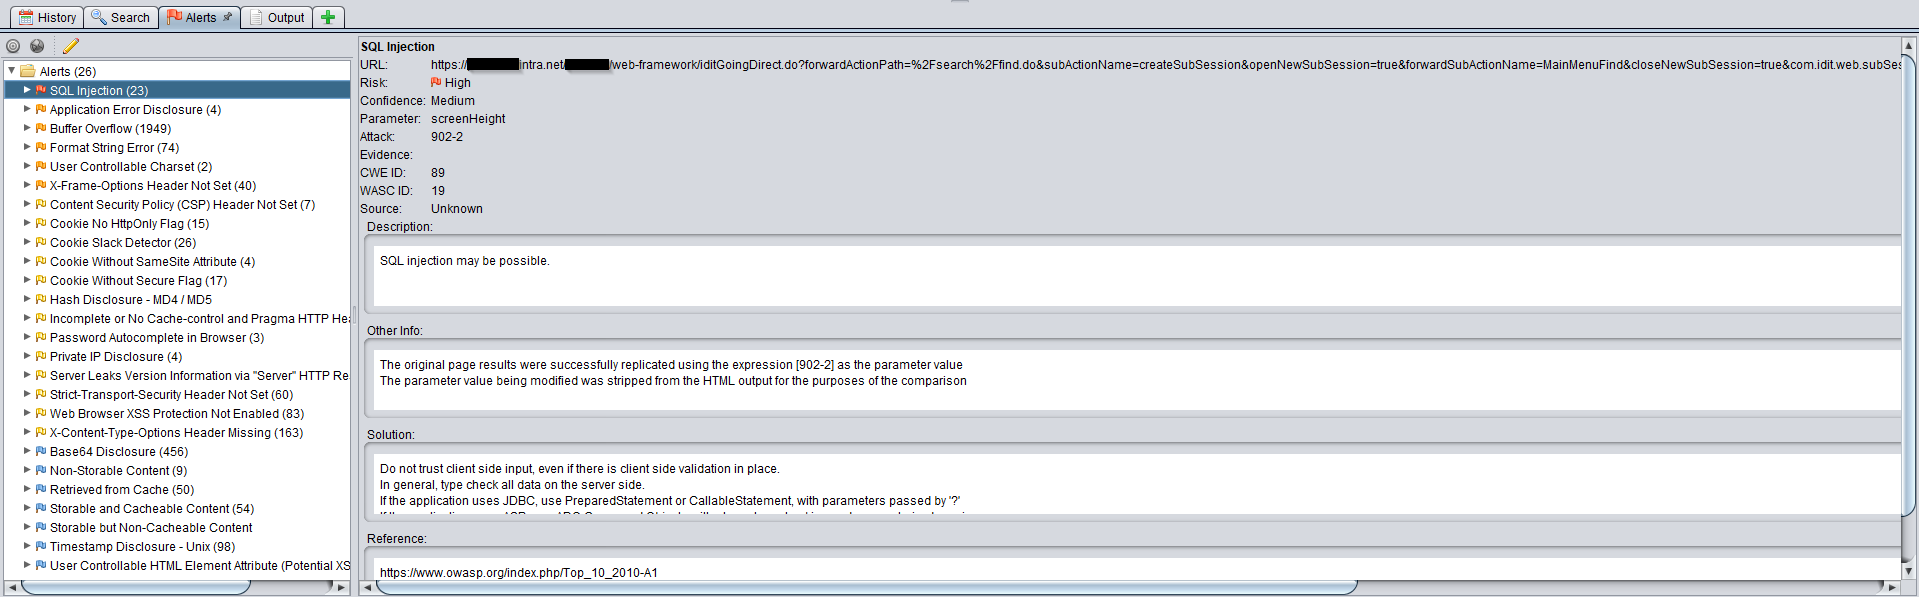
\includegraphics[width=\paperwidth]{images/zap_res}}
\end{figure}

Les résultats étaient plutôt modérés une fois les faux positifs exclus (voir un aperçu dans la figure~\ref{fig:zap_res}) : l'application est en Java ce qui limite d'emblée les possibilités de buffer overflow, nous n'avons pas réussi à reproduire les SQLi et XSS suspectées par ZAP, etc. Les divulgations d'informations techniques étaient légion en revanche et donc le problème le plus facile à remarquer et reproduire. 

Un des objectifs de l'audit était de comparer aux années précédentes pour avoir une mesure de l'évolution de l'application, et celle-ci était très positive : le nombre de failles de sécurité a drastiquement réduit, certaines ont entièrement disparu et d'autres énormément diminué en termes d'occurrences. On verra plus loin que ce constat s'applique aux autres aspects de l'audit aussi. 

\subsection{Performance}
Cette partie de l'audit s'est basée sur JMeter et nmon (et SoapUI dans une moindre mesure, mais ce dernier ne permet pas de faire de mesures et il nous a simplement servi à mettre en place les requêtes envoyées par JMeter). 

JMeter, une fois pris en main, est assez simple à configurer pour les fonctionnalités qui nous intéressaient. Un employé de l'entreprise cliente nous a assisté et a joué des scénarios qu'il rencontrait dans son travail de tous les jours, que nous enregistrions avec JMeter configuré comme un proxy. À quelques éléments de configuration près (e.g. la génération procédurale de nouveaux comptes sur l'intranet comme dans l'image~\ref{fig:jmeter_user} où un compteur \verb|${generated_login}| est maintenu par JMeter et sert à générer des identifiants uniques) il n'y avait plus qu'à automatiser l'exécution des scénarios de test, et attendre puis analyser les résultats. 

\begin{figure}
  \centering
  \caption{Génération procédurale d'utilisateurs par JMeter}
  \label{fig:jmeter_user}
  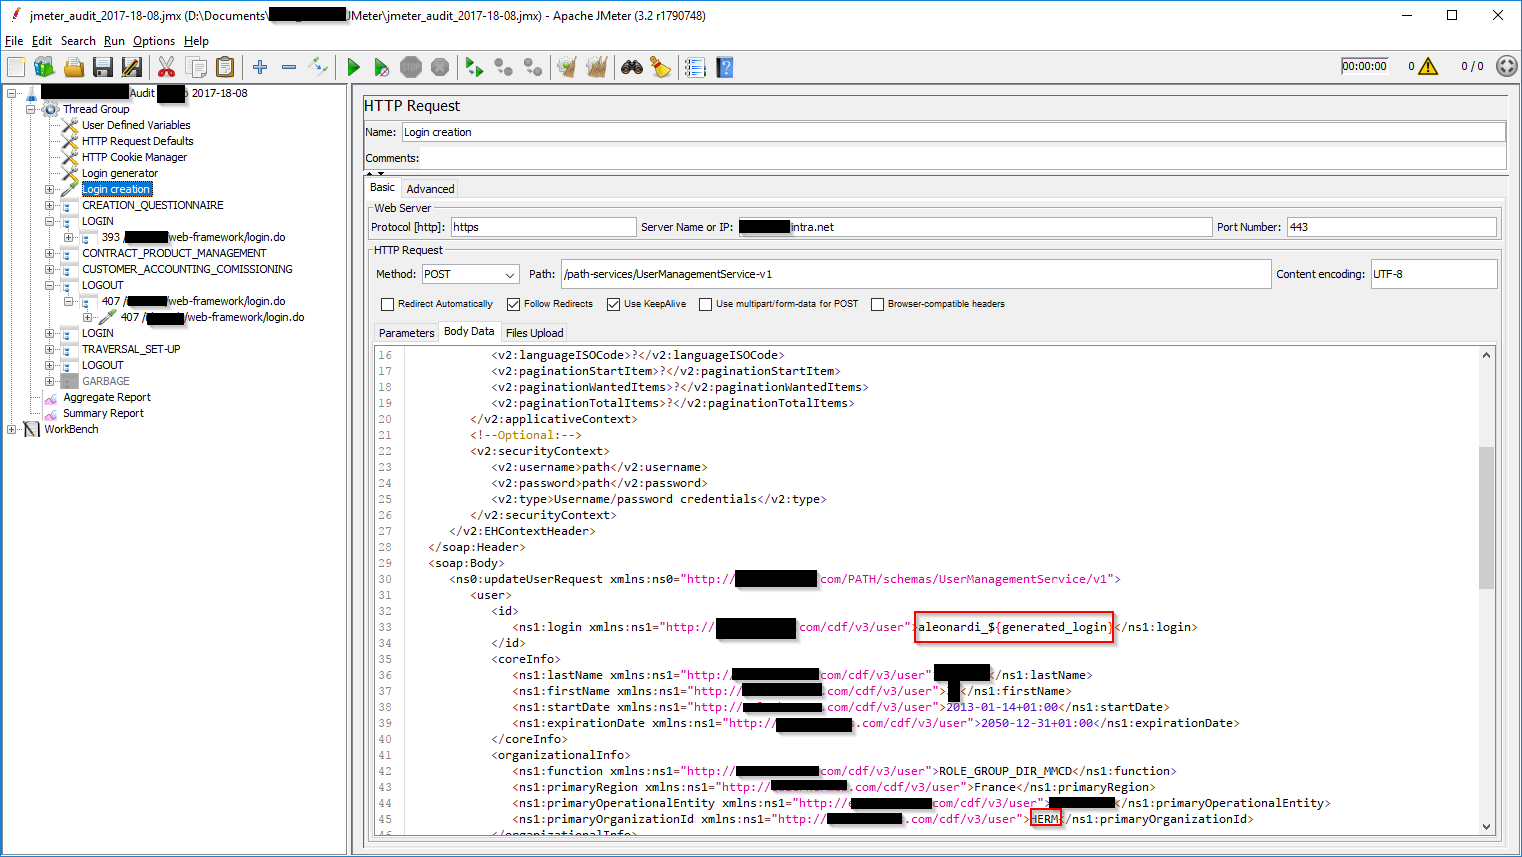
\includegraphics[width=\textwidth]{images/jmeter_login}
\end{figure}

L'automatisation en question est triviale : on peut voir le panneau concerné dans l'image~\ref{fig:jmeter_config}. On renseigne des informations telles que le nombre d'utilisateurs (correspondant à un thread qui va exécuter les tests en boucle), le nombre de tours de boucle que fait chaque utilisateur, la durée de la montée en charge (c'est-à-dire la fréquence de création des utilisateurs), etc. 

\begin{figure}
  \centering
  \caption{Configuration des tests joués par JMeter}
  \label{fig:jmeter_config}
  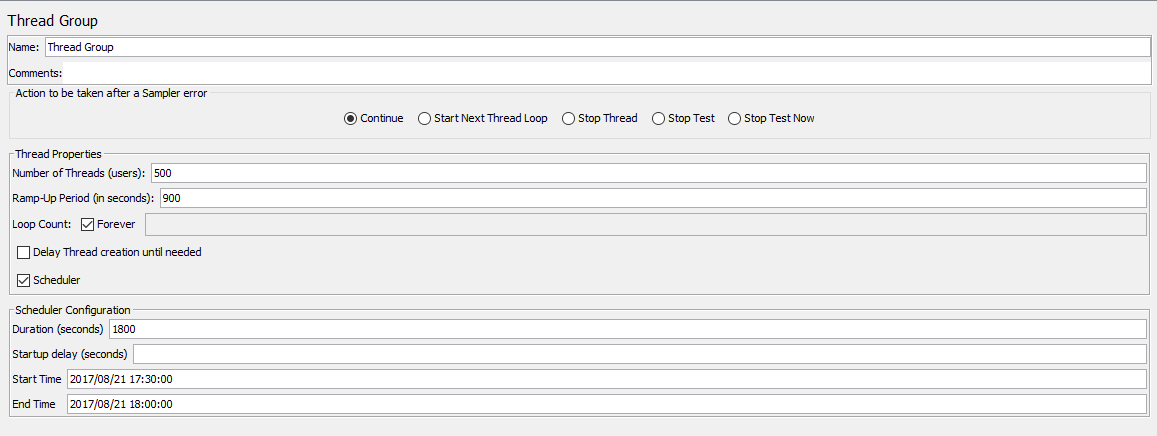
\includegraphics[width=\textwidth]{images/jmeter_config}
\end{figure}

La véritable valeur ajoutée que nous apportons arrive au moment de choisir les valeurs pour ces tests, et d'en interpréter les résultats. Outre des cas ne faisant intervenir que peu d'utilisateurs simultanés, que nous avons joué à titre d'exemple pour prendre en main l'outil, les deux configurations importantes sont une à 100 utilisateurs simultanés (ce qui est plus que l'affluence réelle que doit supporter l'application, mais reste vraisemblable) et une à 500 utilisateurs (pour voir à quel moment précis le serveur devenait surchargé et inaccessible). 

JMeter produit des résultats très complets et, avec la configuration par défaut, presque illisibles car affichant trop d'informations. La capture d'écran~\ref{fig:jmeter_res} est un extrait que j'ai affiné des temps de réponse du serveur en fonction du temps écoulé : les temps affichés peuvent sembler extrêmement longs (le pic est à 417s environ) mais ils sont à relativiser car chaque courbe représente un ensemble d'opérations (une \emph{chaîne fonctionnelle}). 

\begin{figure}
  \centering
  \caption{Extrait des résultats fournis par JMeter, pour le test à 100 utilisateurs}
  \label{fig:jmeter_res}
  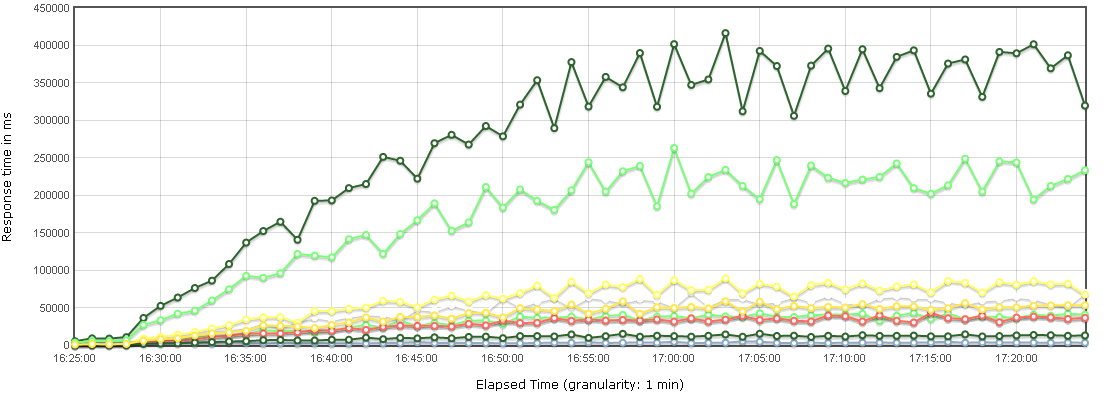
\includegraphics[width=\textwidth]{images/jmeter_res}
\end{figure}

Malgré cela, les temps restent longs : compte tenu des opérations que regroupe chaque chaîne fonctionnelle, plus de cinq minutes pour la plus longue d'entre elles représente un temps excessif mais qui ne rend pas l'application inutilisable. Notre objectif, dans cet audit, était de mettre en avant les éléments les plus consommateurs de temps, mais pas d'analyser le code et fournir des suggestions d'amélioration. Le rapport d'audit s'est donc arrêté à souligner quels éléments faisaient goulot d'étranglement, laissant la charge d'améliorer la situation au client. 

J'ai parlé plus tôt d'un autre outil : nmon. Il nous a servi à surveiller la consommation de ressources (mémoire et CPU) du seveur, ce qui était intéressant pour les corréler aux données de JMeter mais ne nous a pas apporté d'information neuve. Un exemple de résultats de nmon : la capture~\ref{fig:nmon_res}.

\begin{figure}
  \centering
  \caption{Extrait des résultats fournis par nmon, pour le test à 500 utilisateurs : noter la saturation du CPU à partir de 16h}
  \label{fig:nmon_res}
  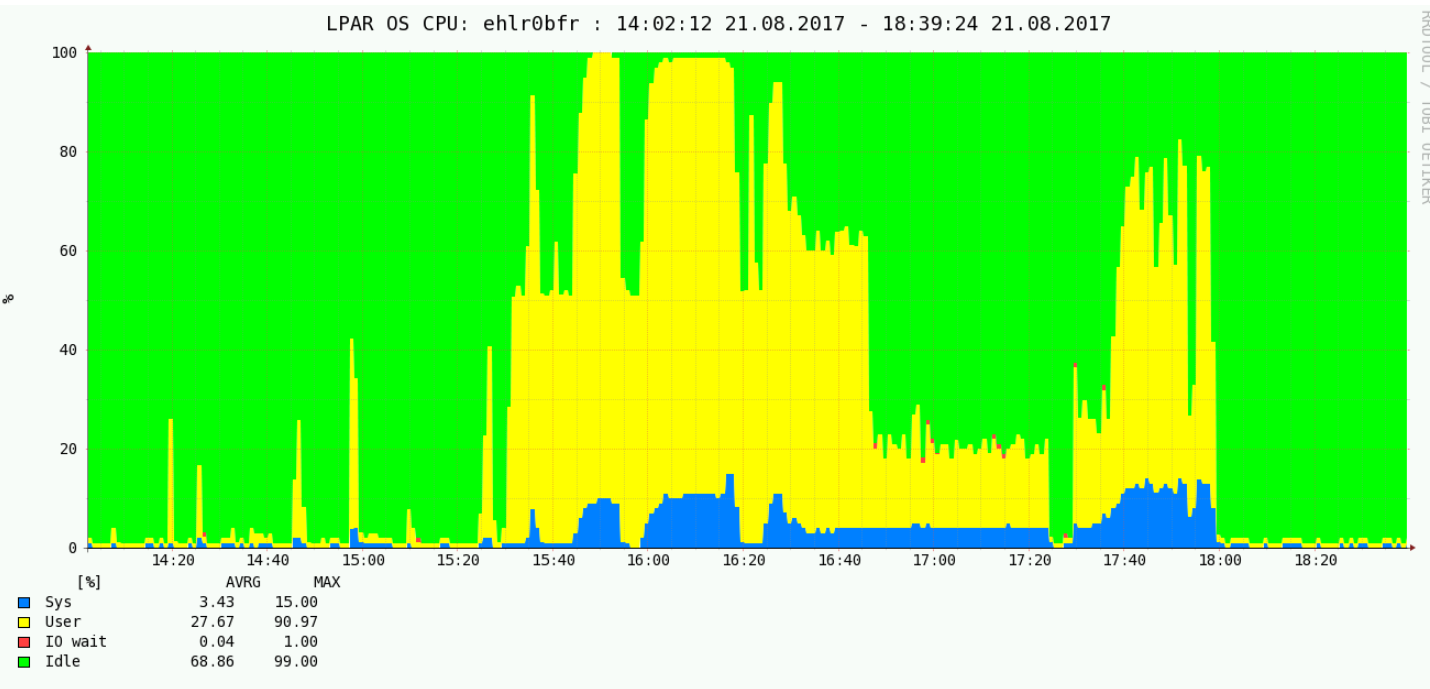
\includegraphics[width=\textwidth]{images/nmon_res}
\end{figure}

Une fois encore nous voulions mettre en relief les changements survenus depuis la précédente itération de l'audit, et encore une fois ils étaient positifs : d'une part les temps de réponse, bien qu'encore longs, se sont nettement améliorés (la page d'accueil, après la connexion, pouvait prendre plus d'une minute à charger).

Qui plus est, la résistance à la charge est sans commune mesure : le serveur était, dans l'audit précédent, surchargé par 100 utilisateurs simultanés (le taux de réponse aux requêtes diminuait dés 50 utilisateurs). Dans l'audit auquel j'ai participé, la première chute en temps de réponse se fait à 8 minutes soit environ à 260 utilisateurs simultanés. 

\subsection{Qualité}
Pour partie, cet aspect de l'audit n'a pas encore été traité au moment où je rédige ce rapport. Je suis entrain de réaliser des analyses de code avec le chef de projet sous la tutelle de qui je travaille et il est trop tôt pour donner des résultats. 

Il est néanmoins possible de présenter ce que le client demande précisément en la matière :
\begin{itemize}
  \item analyser un certain nombre de problèmes récemment corrigés (les \emph{root causes}) et statuer sur la stabilité des corrections apportées, sur le fait qu'elles n'oublient pas de cas limite et qu'elles soient faciles à étendre ;
  \item analyser certains aspects du code qui ne correspondent pas à un problème précis mais à des notions plus larges, telles que la duplication de code ou les accès à la base de données. 
\end{itemize}

Pour l'instant, nous avons travaillé sur le point précis des duplications de code, avec SonarQube. L'outil propose, parmi ses règles par défaut, de trouver les blocs de code dupliqués dans le code. La capture~\ref{fig:sonar_res} montre une partie des résultats : l'application auditée est séparée en deux parties, mais la partie \og interface \fg ici est la plus concernée par les duplications. 

\begin{figure}
  \centering
  \caption{Représentation graphique des relevés de code dupliqué par SonarQube}
  \label{fig:sonar_res}
  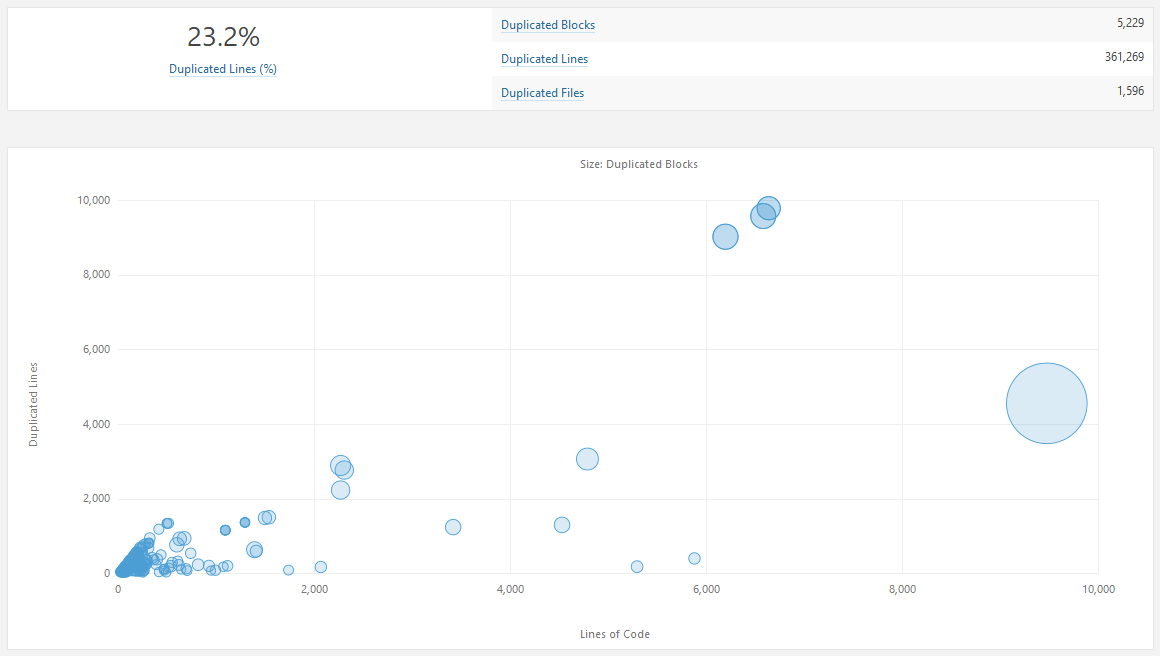
\includegraphics[width=\textwidth]{images/sonar_results}
\end{figure}

Le récapitulatif sur la partie qualité va s'arrêter ici, car l'audit n'est pas assez avancé pour en parler plus avant. La prochaine étape de notre audit, néanmoins, va être de parcourir le code source à l'aide du récapitulatif des commits ayant corrigé les \emph{root causes} et de donner un avis sur les éventuels oublis ou améliorations possibles. 